\section{Methodology}

\subsection{Problem formulation}

We treat aerodynamic shape design as an \emph{inverse} problem: given a target surface-pressure
distribution $C_p(x/c)$, produce a closed 2D boundary shape that realises it. The boundary is
represented as a radial field $r(\theta)$ sampled at the surface nodes, and the design target is
summarised by a conditioning context $c$ derived from $C_p(x/c)$. The map from target pressure to
shape is \emph{one-to-many}: distinct boundaries can carry near-identical pressure curves, so there
is no single correct output to regress towards. A deterministic regressor, forced to average over
this fibre, would collapse the valid set to a blurred mean shape. A generative model instead learns
the conditional distribution $p(r(\theta) \mid c)$, sampling individual valid shapes for a given
target --- which is why we adopt a conditional generative formulation rather than direct regression.

\subsection{Shape representation}

We diffuse the boundary as a radial field $r(\theta)$ sampled at the surface nodes, organising those
nodes into a boundary graph with bidirectional ring edges so each node exchanges messages with its
two ring neighbours. The data pipeline supports several coordinate parameterisations of the same
boundary --- direct-Cartesian $(x, y)$, raw radial, and scale-normalised radial --- and we adopt the
scale-normalised radial field as the diffusion target.
This choice is principled rather than incidental. A single scalar per node is a minimal,
well-conditioned one-dimensional target on the ring, avoiding the two coupled channels of a
Cartesian parameterisation. It exposes $r(\theta)$ directly to a second-difference (curvature)
diagnostic, so surface smoothness can be both measured and, where useful, penalised. Normalising by
scale further decouples shape from absolute size, focusing the model on morphology. The same radial
target was first validated on canonical shapes in a preliminary study (Section~4.1), where radial
diffusion on a ring graph reproduced target shape distributions, and was carried unchanged into the
aerodynamic setting.

\subsection{Denoising diffusion model}

The generator is a denoising diffusion probabilistic model (DDPM) \cite{ho2020ddpm} operating on
the graph node features. The forward process corrupts a clean shape $x_0 = r(\theta)$ with Gaussian
noise over $T$ steps; in closed form the marginal at step $t$ is

\begin{equation}
  q(x_t \mid x_0) = \mathcal{N}\!\left( x_t ;\, \sqrt{\bar{\alpha}_t}\, x_0,\, (1-\bar{\alpha}_t) I \right),
\end{equation}

where $\bar{\alpha}_t$ is the cumulative product of the noise schedule. We use a cosine
$\bar{\alpha}_t$ schedule \cite{nichol2021improved}, which spends fewer steps in the near-pure-noise
regime than the original linear schedule and so allocates more reverse steps to the low-noise regime
where fine geometric detail emerges. A learned network reverses the process, denoising
$x_T \sim \mathcal{N}(0, I)$ back to a shape, and is trained to predict the injected noise
$\varepsilon$ under the standard simple loss

\begin{equation}
  L = \mathbb{E}_{t, x_0, \varepsilon} \left[ \lVert \varepsilon - \varepsilon_\theta(x_t, t, c) \rVert^2 \right],
\end{equation}

an MSE between the true and predicted noise, with $c$ the conditioning context. All schedule buffers
(\texttt{betas}, \texttt{alphas\_cumprod}, and derived quantities) are owned by a
\texttt{NoiseSchedule} module and registered as module buffers, so they move with the device and are
saved inside checkpoints, guaranteeing that training and sampling share an identical schedule.

\begin{figure}[t]
  \centering
  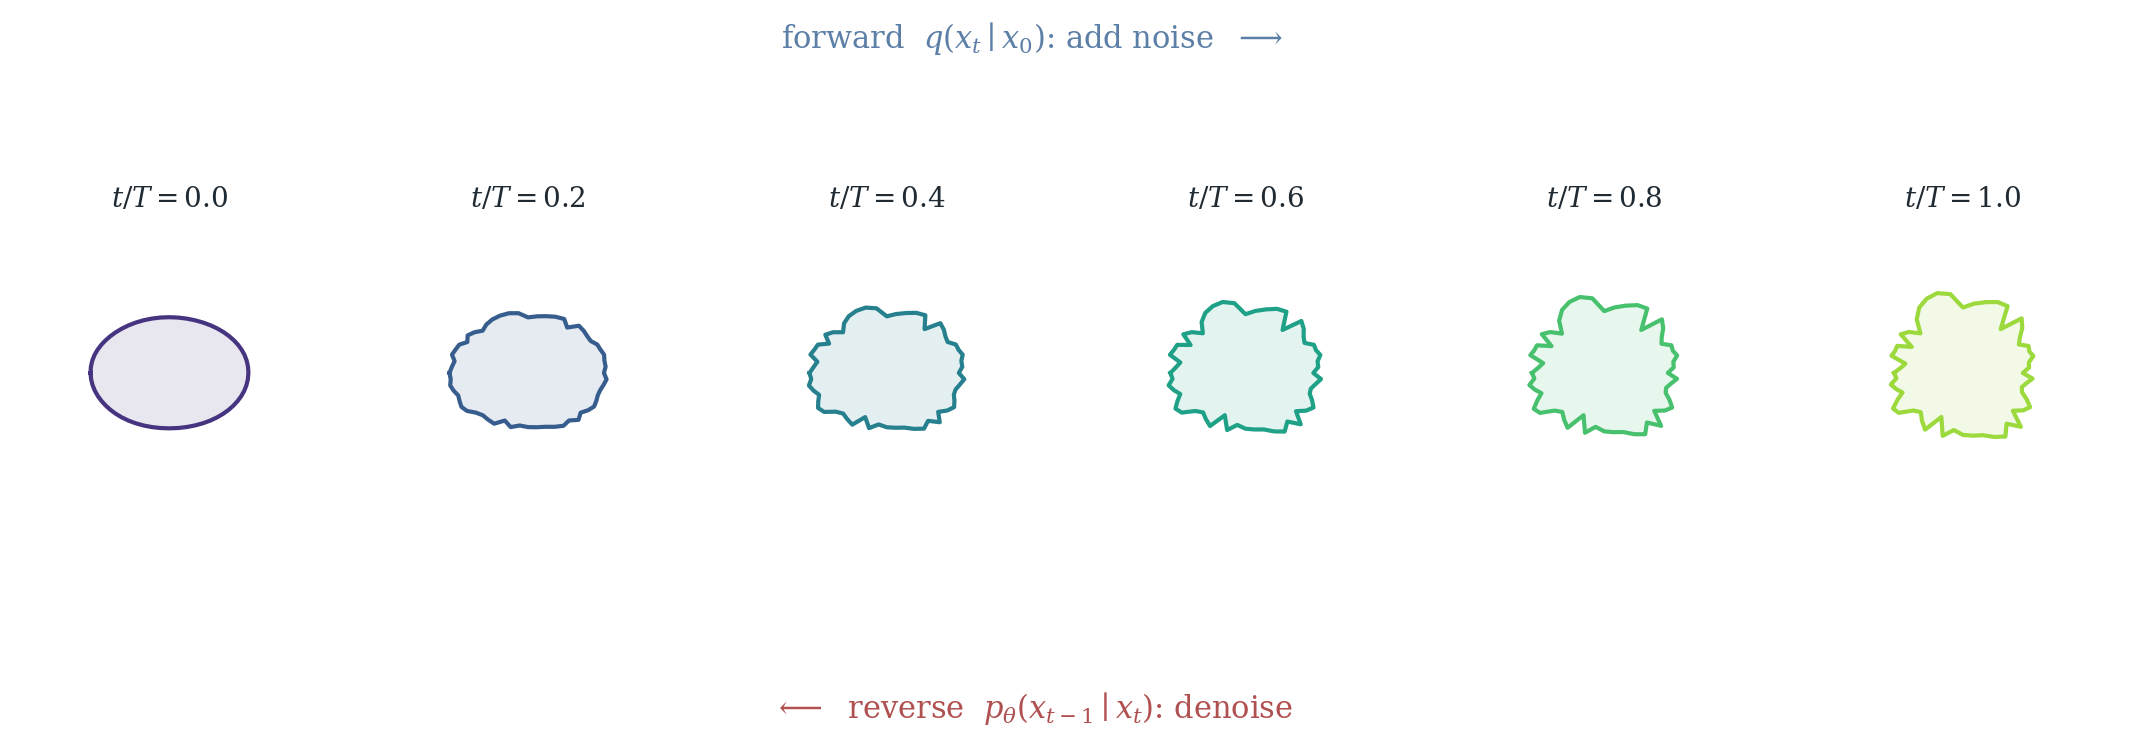
\includegraphics[width=0.95\linewidth]{report_diffusion_process.png}
  \caption{Forward and reverse diffusion on the radial field $r(\theta)$ of a real generated boundary.
  The forward process $q(x_t \mid x_0)$ progressively corrupts a clean shape (left) toward isotropic
  noise (right) along the cosine schedule; the learned reverse process denoises back, recovering
  surface detail in the final low-noise steps.}
  \label{fig:diffusion-process}
\end{figure}

\subsection{Graph-network score model}

The score network $\varepsilon_\theta$ stacks $N$ Battaglia-style graph-network blocks
\cite{battaglia2018relational}, each applying the canonical three-stage update ---
$\phi^e \to \phi^v \to \phi^u$ --- and aggregating messages along the bidirectional ring edges of
the boundary. The key design choice is how time and conditioning enter the network: the timestep is
mapped through a sinusoidal embedding, and both this embedding and the conditioning vector are
injected \emph{once} into the per-graph global attribute $u$, rather than being concatenated onto
every node. They then propagate to the nodes through the $\phi^u \to \phi^v$ message-passing
pathway, so a single per-graph signal conditions all nodes consistently and the per-node feature
stays a single radial channel. The model is implemented under a strict one-way package dependency
DAG (\texttt{building\_blocks/} $\to$ \texttt{model/}, with \texttt{data/} independent of both),
keeping the score architecture decoupled from data handling.

\begin{figure}[t]
  \centering
  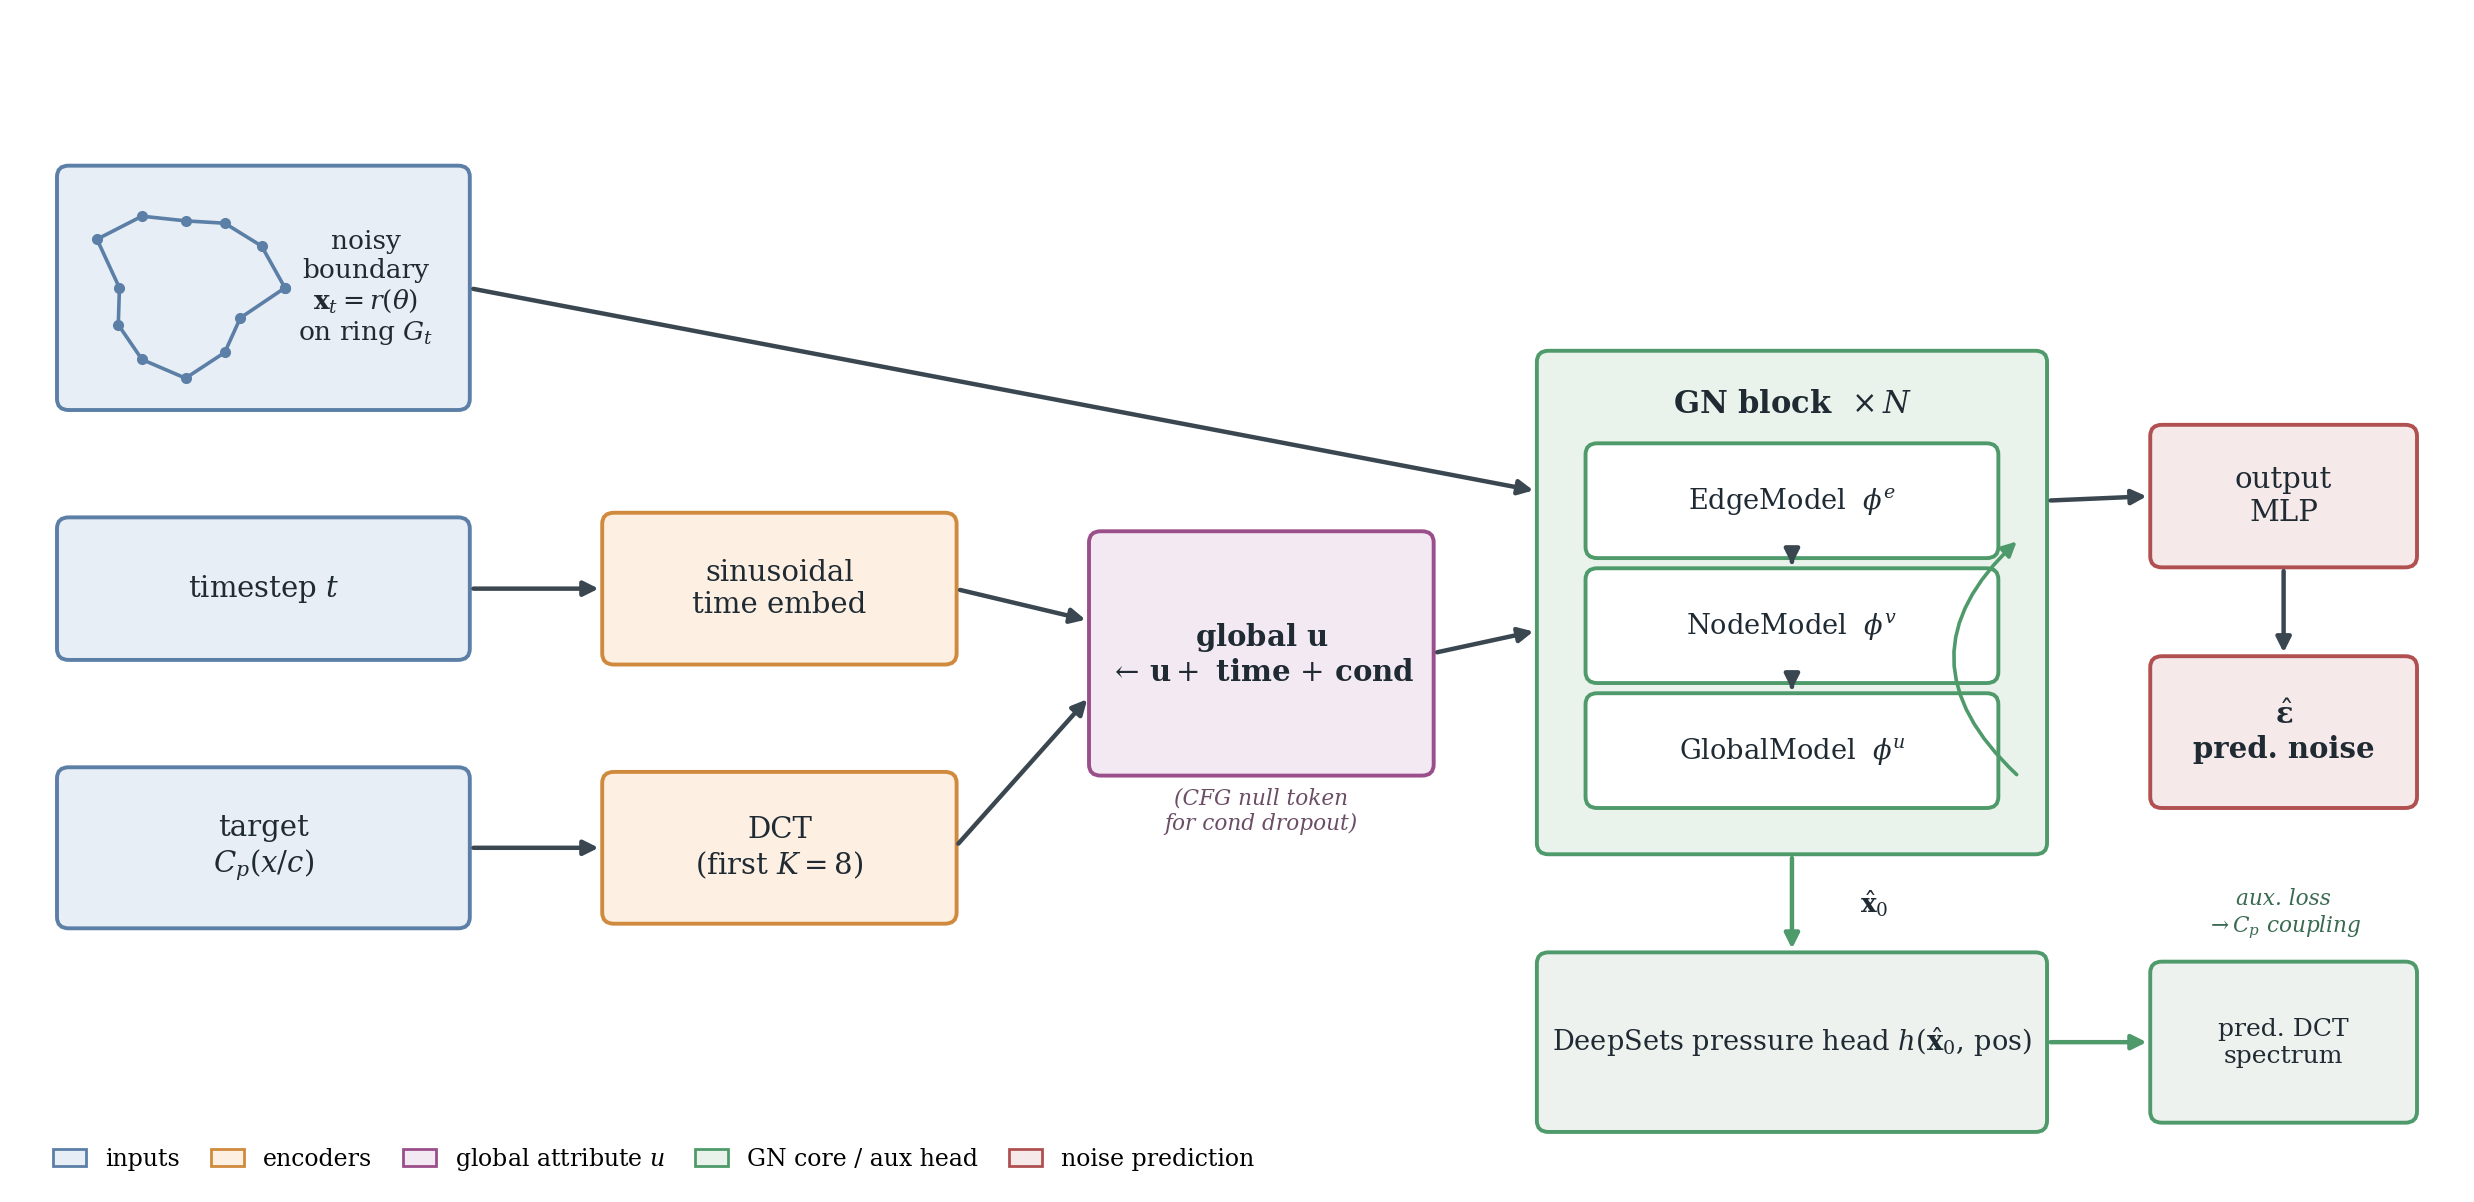
\includegraphics[width=0.8\linewidth]{report_architecture.png}
  \caption{Architecture of the score network $\varepsilon_\theta$. The diffusion timestep (via a
  sinusoidal embedding) and the DCT pressure-conditioning vector are summed once into the per-graph
  global attribute $u$, which feeds the $N\times$ stack of graph-network blocks
  ($\phi^e \to \phi^v \to \phi^u$) operating over the bidirectional ring edges; a
  jointly-trained auxiliary DeepSets pressure head reads the denoised shape to predict its pressure
  spectrum (detailed in Section~3.5).}
  \label{fig:architecture}
\end{figure}

\subsection{Pressure conditioning}

The target pressure curve is encoded compactly: we take the first $K=8$ type-II discrete cosine
transform (DCT) coefficients of the steady-mean $C_p(x/c)$. This yields a fixed-size conditioning
vector that is independent of the surface node count and captures the smooth, low-frequency
morphology of the pressure curve in a handful of numbers. Encoding alone, however, does not force
the model to respect physics. To tie geometry to pressure, a DeepSets pressure head
\cite{zaheer2017deepsets} $h(\hat{x}_0, \mathrm{pos}) \to \mathbb{R}^K$ is trained jointly with
the score network: from the denoised shape it must predict the DCT spectrum of the pressure that the
\emph{generated} shape would actually produce. Its prediction error supplies an auxiliary gradient
that couples the generated geometry to its implied pressure, forcing the model to learn the forward
shape$\to$pressure map rather than memorise training shape--pressure pairs. The DeepSets form is
chosen because it is permutation-invariant over the unordered set of surface nodes, matching the
symmetry of the boundary.

\begin{figure}[t]
  \centering
  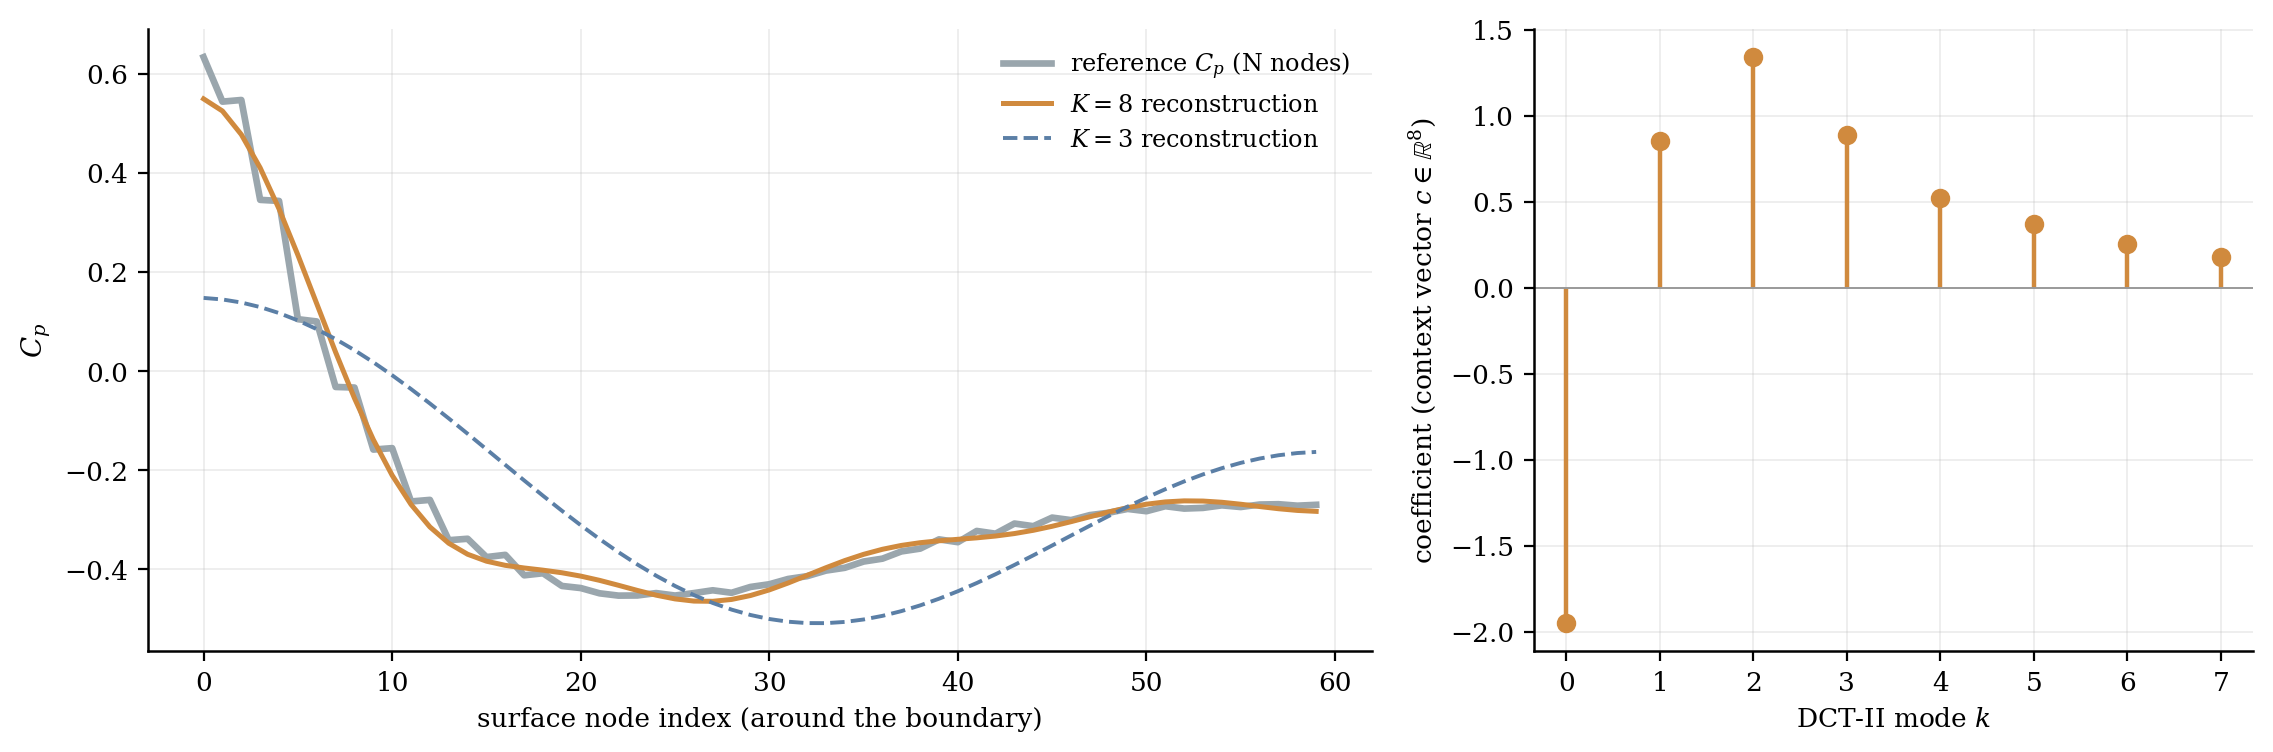
\includegraphics[width=0.85\linewidth]{report_dct_encoding.png}
  \caption{A real reference pressure sequence (grey) and its truncated DCT-II reconstruction. Eight
  modes ($K=8$, orange) recover the pressure morphology closely, while three modes (blue dashed) are
  visibly too coarse, motivating $K=8$ as a compact, node-count-independent conditioning vector.
  Right: the eight coefficients constituting the context vector $c$.}
  \label{fig:dct-encoding}
\end{figure}

\begin{figure}[t]
  \centering
  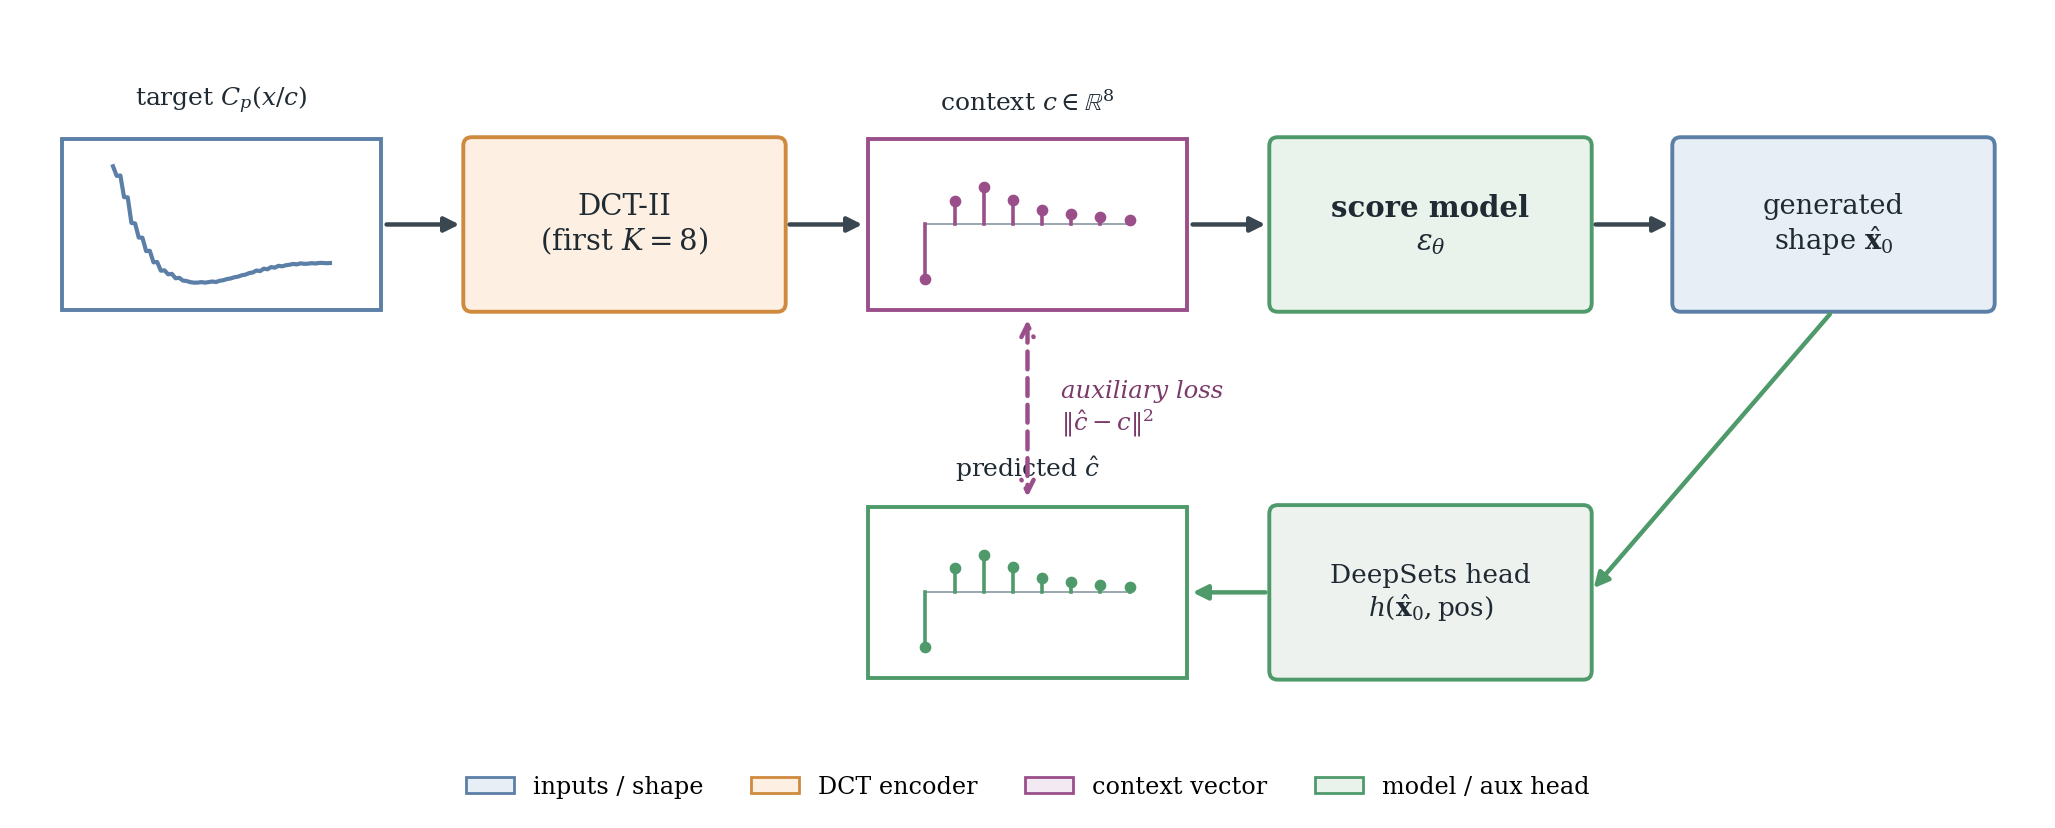
\includegraphics[width=0.95\linewidth]{report_conditioning_pipeline.png}
  \caption{The pressure-conditioning data flow. The target $C_p(x/c)$ is DCT-encoded into the
  fixed-size context $c$ that conditions the score model; the jointly-trained DeepSets head reads the
  generated shape and predicts its pressure spectrum $\hat{c}$, and the auxiliary loss
  $\lVert \hat{c} - c \rVert^2$ couples generated geometry back to pressure.}
  \label{fig:conditioning-pipeline}
\end{figure}

\subsection{Inference guidance}

At sampling time the conditioning signal is amplified with classifier-free guidance \cite{ho2022cfg}.
During training the condition is randomly dropped and replaced by a learnable null token, so the
same network learns both conditional and unconditional noise prediction. At inference the two
predictions are combined,

\begin{equation}
  \varepsilon = (1 + w)\cdot\varepsilon_\mathrm{cond} - w\cdot\varepsilon_\mathrm{uncond},
\end{equation}

with guidance weight $w$ (here $w=3.0$), pushing samples toward the target without a separate
classifier. The tested alternative is Diffusion Posterior Sampling \cite{chung2023dps}, which
instead adds a likelihood gradient from the jointly-trained pressure head to steer the reverse
process toward the measured target; its effect on out-of-distribution targets is reported in the
Results.

\subsection{Independent CFD validation solver}

Generated shapes are graded by an independent computational fluid dynamics solve rather than by the
model's own pressure head. The validation loop is a 2D incompressible lattice-Boltzmann solve
\cite{kruger2017lbm} built on OpenLB \cite{latt2021openlb}. The generated boundary polygon is
stamped into the lattice as a solid via a winding-number signed-distance indicator, giving a curved
Bouzidi no-slip body wall; the domain spans a velocity inlet, free-stream-velocity Dirichlet
conditions on the top and bottom walls, and a pressure outlet, with the channel height $H$ taken
from the dataset and the body centred at the half-height $H/2$. A graded sponge / absorbing layer
\cite{xu2013sponge} sits upstream of the outlet to suppress reflected acoustic waves that would
otherwise contaminate the measured field. The decisive property is independence: the solver measures
the time-averaged surface $C_p(x/c)$ from first principles and never sees the diffusion model or its
pressure head. Because the grading physics shares no component with the generator, a high
measured-versus-target correlation is a genuine physical confirmation of inverse design, not a
surrogate grading itself.

\begin{figure}[t]
  \centering
  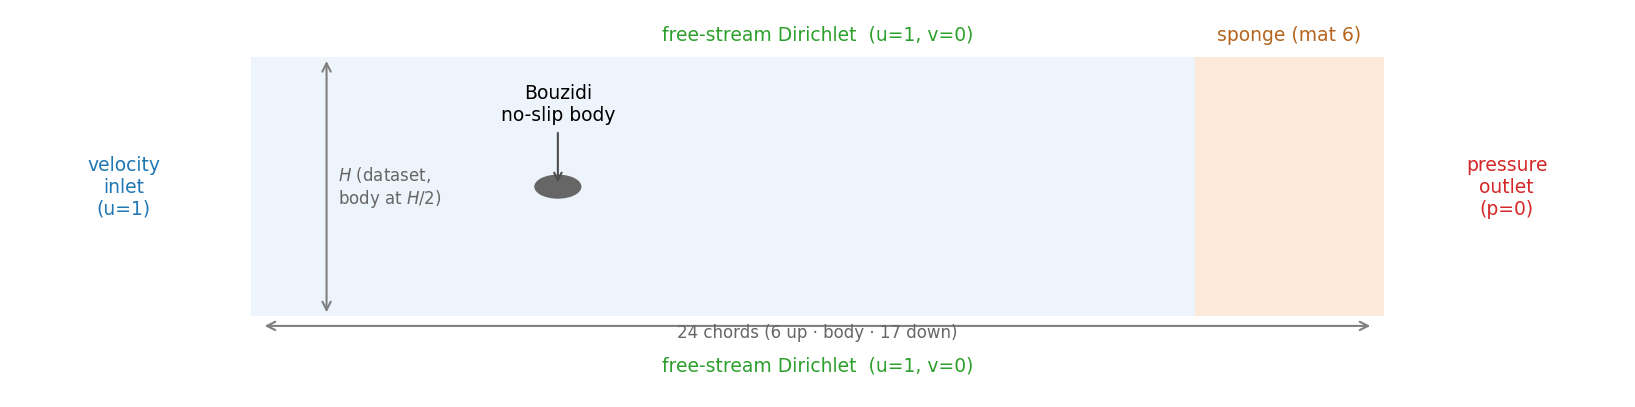
\includegraphics[width=0.8\linewidth]{EXP-043_domain_schematic.png}
  \caption{Schematic of the 2D lattice-Boltzmann validation domain: a velocity inlet, free-stream
  Dirichlet top and bottom walls, the stamped solid body with a curved Bouzidi no-slip wall centred
  at the dataset channel half-height $H/2$, and a pressure outlet preceded by a graded sponge layer.}
  \label{fig:domain-schematic}
\end{figure}

\paragraph{Key implementation details.} The solver is built on OpenLB 1.9.0 with a \texttt{D2Q9}
lattice and plain BGK collision (the target $Re$ 500--1000 is laminar, so no turbulence model). Five
elements fix the physics, and the code below shows how each is set up.

\paragraph{Reynolds number via viscosity.} The characteristic free-stream speed is held fixed at
$U = 1$ and the chord at $L = 1$; Reynolds number enters only through the physical viscosity
$\nu = U L / Re$, so $Re$ is decoupled from the inlet velocity. The unit converter is seeded from the
spatial resolution and the lattice relaxation time $\tau = 0.545$ (just above the BGK stability floor
of 0.5):

\begin{lstlisting}[style=cpp]
lattice.setUnitConverter<UnitConverterFromResolutionAndRelaxationTime<T,DESCRIPTOR>>(
    resolution,                          // voxels per chord  (RES ~ 0.2*Re for stability)
    latticeRelaxationTime,               // tau = 0.545   (> 0.5 BGK floor)
    charPhysLength,                      // L = chord = 1
    charPhysVelocity,                    // U = 1 m/s   (fixed)
    charPhysVelocity*charPhysLength/Re,  // nu = U*L/Re  <- Reynolds enters here
    physDensity);
\end{lstlisting}

Because the Mach number $\mathrm{Ma} = U_\mathrm{lattice}/c_s$ must stay $\lesssim 0.1$ for
incompressibility while the cell viscosity falls with $Re$, the grid resolution is scaled with Reynolds
number, $\mathrm{RES} \approx 0.2\,Re$, to keep the lattice viscosity in a stable band across the whole
regime.

\paragraph{Domain and channel height.} The domain spans $6 + 1 + 17 = 24$ chords streamwise (inlet 6
chords upstream of the body, outlet 17 downstream); the cross-stream extent is the dataset channel
height $H$ (5--6), and the body is centred at the half-height $H/2$, matching the dataset blockage ratio
rather than being free-chosen:

\begin{lstlisting}[style=cpp]
const T physDeltaX  = chord / resolution;
const T physLengthX = (upstreamChords + 1 + downstreamChords) * chord;  // 6 + 1 + 17 chords
const T physLengthY = H + physDeltaX;                    // channel height H (dataset 5-6)
const T shiftY      = (physLengthY / 2) - body.centroid[1];   // body centred at H/2
\end{lstlisting}

The channel height is a required input with no default --- an omitted \texttt{--CHANNEL\_HEIGHT} aborts
the run (a $-1.0$ sentinel $+$ a guard), so a wrong-domain run cannot pass silently.

\paragraph{Material map and boundary conditions.} The geometry is tagged with six material numbers ---
bulk fluid (1), free-stream top/bottom (2), velocity inlet (3), pressure outlet (4), the body (5), and
an absorbing sponge band (6) --- and each gets its dynamics or boundary condition:

\begin{lstlisting}[style=cpp]
dynamics::set<BGKdynamics>(lattice, geometry.getMaterialIndicator({1}));  // bulk
boundary::set<boundary::InterpolatedVelocity>(lattice, geometry, 3);      // inlet  (U, 0)
boundary::set<boundary::InterpolatedVelocity>(lattice, geometry, 2);      // free-stream top/bottom
boundary::set<boundary::InterpolatedPressure>(lattice, geometry, 4);      // outlet p = 0
setBouzidiBoundary(lattice, geometry, 5, *placedShape);                   // curved no-slip body
\end{lstlisting}

\paragraph{Body stamping.} The generated boundary polygon is turned into a solid by a hand-written
signed-distance indicator: the sign comes from a winding-number point-in-polygon test (robust for
non-convex shapes) and the magnitude from the nearest-edge distance, giving the true signed distance
(negative inside) that the curved Bouzidi wall reconstruction needs:

\begin{lstlisting}[style=cpp]
const T sign = (windingNumber % 2 == 1) ? -1 : +1;   // odd crossings => inside
return sign * nearestEdgeDistance;                   // negative inside, positive outside
\end{lstlisting}

\paragraph{Surface $C_p$ from a time-averaged field.} Because the flow sheds vortices, a single-step
pressure readout is meaningless; the solver discards the start-up transient and accumulates a
time-averaged pressure field over a window spanning many shedding periods. The surface $C_p(x/c)$ is
then probed half a cell outside each boundary node along its outward normal, and referenced to the
undisturbed free-stream static pressure (sampled $0.4\,H$ above the body) rather than the outlet gauge,
so the stagnation point reads $C_p \approx 1$:

\begin{lstlisting}[style=cpp]
const T qInf = 0.5 * rho * U * U;                     // dynamic pressure
const Vector<T,2> probe{ node[0] + 0.5*dx*nrm[0],     // 0.5*dx outside the surface,
                         node[1] + 0.5*dx*nrm[1] };   // along the outward normal
Cp = (p_timeAveraged(probe) - p_inf) / qInf;          // p_inf from a free-stream probe
\end{lstlisting}

A graded sponge / absorbing layer \cite{xu2013sponge} (material 6) just upstream of the outlet, together
with rest-initialisation and a smooth inlet velocity ramp, suppresses reflected pressure waves so the
averaging window sees a clean periodic signal.

\subsection{Dataset}

Training data is the pOnEllipse dataset \cite{lino2022msgnn}: 2D incompressible flow around an
elliptical cylinder of major-axis length 1 (semi-major 0.5), with variable minor axis $b$ and
channel height $H$, at Reynolds numbers 500--1000 --- the laminar vortex-shedding regime. It
comprises 5701 training simulations, each storing per-surface-node coordinates together with 101
unsteady pressure timesteps, which we collapse to a single steady-mean $C_p$. The per-node HDF5
layout is \texttt{[x, y, Re, H, p0..p100]}. Note that the fourth column $H$ is the channel height
($\approx 5$--6), not angle of attack --- a distinction that matters because mistaking it for AoA
would corrupt the conditioning. The narrow, well-characterised regime makes this dataset a
controlled testbed for inverse design before scaling to higher-Reynolds or 3D flows.

\begin{figure}[t]
  \centering
  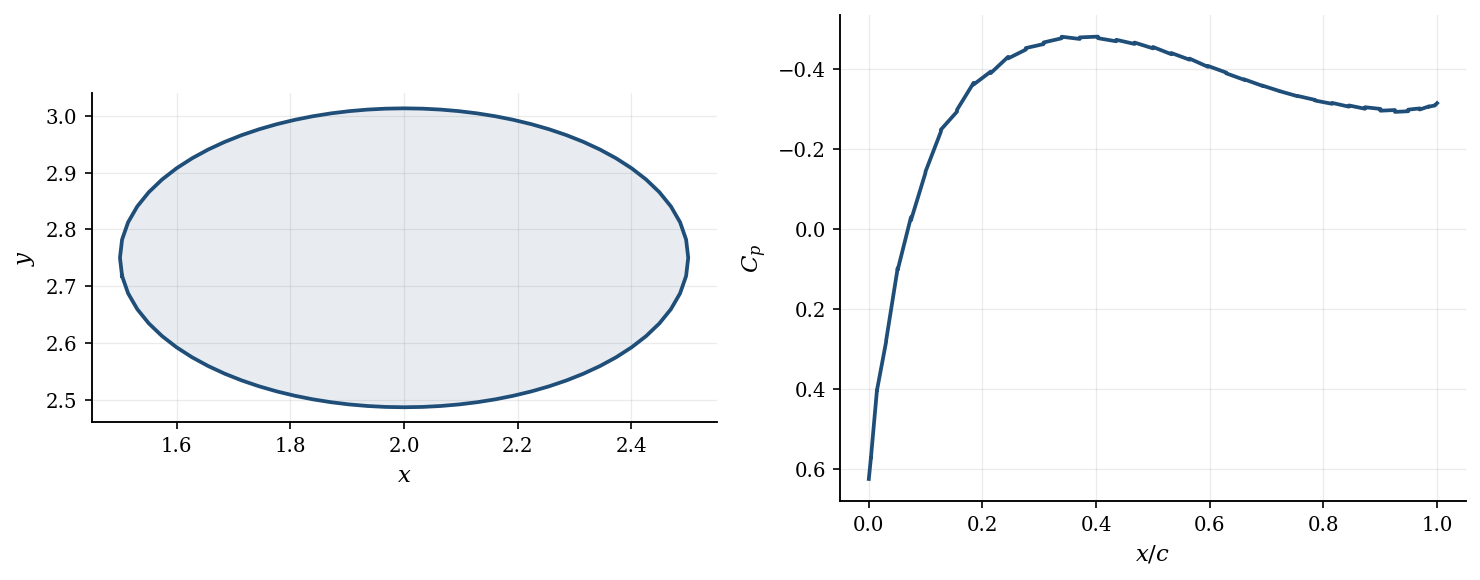
\includegraphics[width=0.8\linewidth]{report_dataset_example.png}
  \caption{An example pOnEllipse training sample: a closed elliptical boundary (left) and its
  corresponding steady-mean surface pressure curve $C_p(x/c)$ (right), the quantity the model is
  conditioned on.}
  \label{fig:dataset-example}
\end{figure}

The dataset spans a two-parameter design space --- Reynolds number $Re$ and semi-minor axis $b$ ---
sampled densely across the laminar regime, with the geometry varying smoothly with $b$.

\begin{figure}[t]
  \centering
  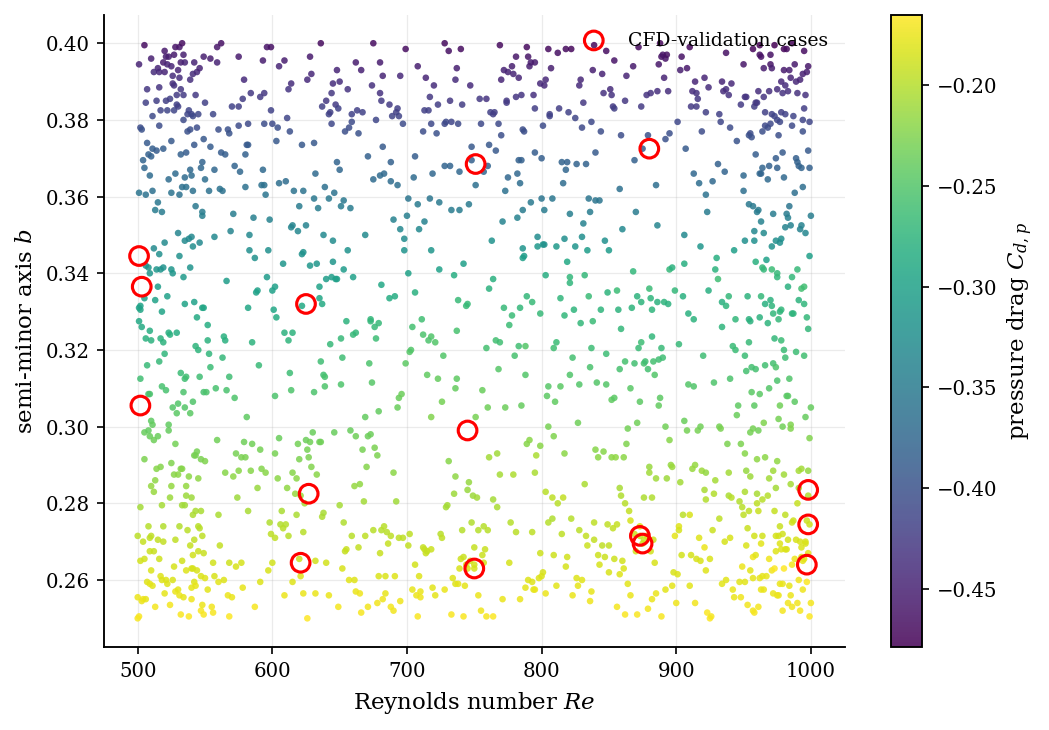
\includegraphics[width=0.7\linewidth]{report_design_space.png}
  \caption{Design-space coverage of the training set: each point is one simulation in the $(Re, b)$
  plane, coloured by its pressure drag. Sampling is dense and near-uniform across the regime; the
  circled points mark the cases later put through the CFD validation loop.}
  \label{fig:design-space}
\end{figure}

The conditioning targets the model sees --- the steady-mean $C_p(x/c)$ curves --- form a structured
family whose morphology is dominated by the minor axis $b$ rather than by $Re$: thinner bodies
(small $b$) develop a deeper suction trough, while $Re$ mainly modulates the wake recovery.

\begin{figure}[t]
  \centering
  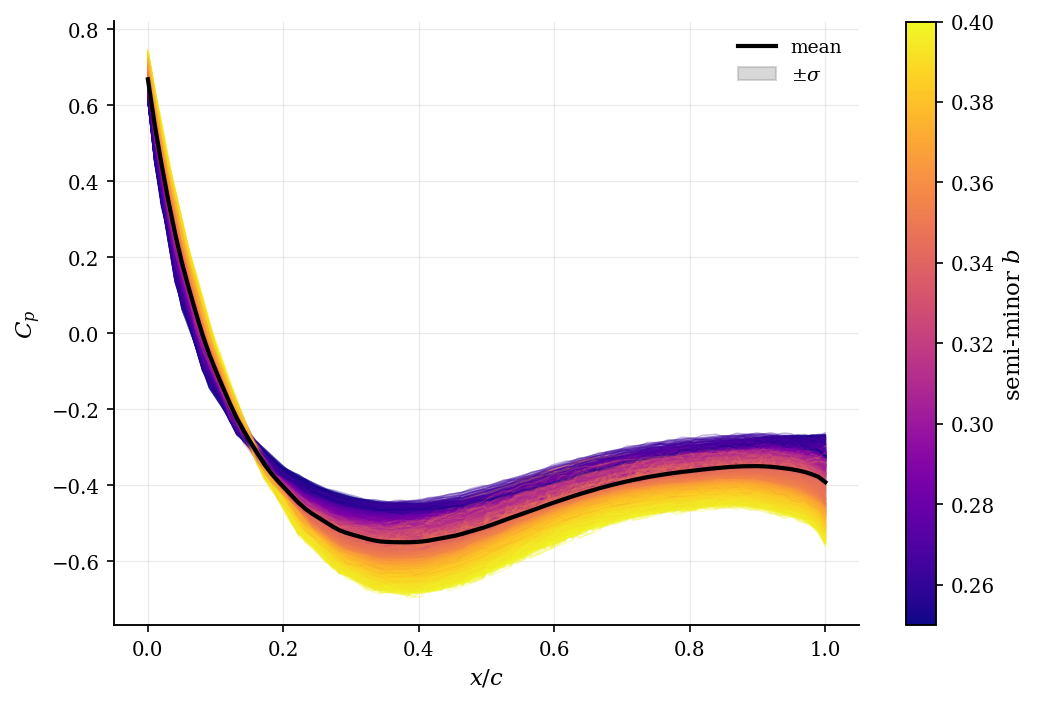
\includegraphics[width=0.7\linewidth]{report_cp_envelope.png}
  \caption{Surface-pressure target distribution across the whole training set, every curve coloured
  by its minor axis $b$ (mean $\pm\,\sigma$ in black). The systematic ordering with $b$ shows that
  $b$ is the principal driver of pressure morphology --- the low-frequency structure the DCT
  conditioning is designed to capture.}
  \label{fig:cp-envelope}
\end{figure}

\subsection{Evaluation metrics}

The headline verdict for inverse design is the \textbf{Pearson correlation} between the
solver-measured $C_p(x/c)$ and the conditioning target: it scores whether the generated shape
reproduces the \emph{shape} of the target pressure curve (its morphology), independently of
amplitude. We report it as the primary metric because the model captures $C_p$ shape, not absolute
magnitude. Alongside it we report the affine slope $a$ and offset $b$ from a linear fit of measured
against target $C_p$, which quantify amplitude calibration; the drag coefficient $C_d$; and the
second-difference roughness of $r(\theta)$, a surface-quality measure where lower is smoother. We
state explicitly that correlation, not absolute amplitude, is the inverse-design verdict --- the
affine slope is reported as a known calibration limitation rather than a pass/fail criterion.

\paragraph{Definition and computation.}
Both metrics are computed on a common abscissa: the solver-measured curve is first interpolated onto
the reference $x/c$ grid so the comparison is point-for-point. Writing the reference samples as $x_i$
and the measured samples as $y_i$ (with means $\bar{x}, \bar{y}$), the Pearson correlation is
\begin{equation}
  \rho \;=\; \frac{\sum_i (x_i - \bar{x})(y_i - \bar{y})}
                  {\sqrt{\sum_i (x_i - \bar{x})^2}\,\sqrt{\sum_i (y_i - \bar{y})^2}},
  \qquad \rho \in [-1, 1],
  \label{eq:pearson}
\end{equation}
the mean-centred, variance-normalised inner product of the two curves. The affine slope and offset are
the least-squares solution of $y \approx a\,x + b$; $a$ is the magnitude scaling and $b$ the constant
offset, and the affine-residual RMS --- the error remaining once the best $a, b$ are removed ---
isolates the part of the mismatch that scaling and offset cannot explain.

\paragraph{Invariance of $\rho$ to the affine fit.}
Pearson correlation is invariant under a positive affine transformation of either variable, which is
exactly why it and the affine fit measure complementary things. Replacing $y$ with the fitted
$a\,y + b$, the covariance scales linearly while the constant drops out,
$\operatorname{cov}(x, a\,y + b) = a\,\operatorname{cov}(x, y)$, and the standard deviation scales by
$|a|$, $\sigma_{a y + b} = |a|\,\sigma_y$, so $\rho(x, a\,y + b) = \operatorname{sign}(a)\,\rho(x, y)$:
for $a > 0$ the slope and offset cancel exactly. Equivalently, the mean-centring in the numerator of
Eq.~\eqref{eq:pearson} annihilates the offset $b$ and the $\sigma$-normalisation in the denominator
annihilates the scale $a$. Correlation is therefore blind, by construction, to overall magnitude and
offset, grading only the \emph{shape} of the pressure distribution, while the affine slope $a$ captures
exactly what $\rho$ discards. The two are reported together and fail independently: a result such as
$\rho \approx 0.999$ with $a \approx 1.87$ reads as ``near-perfect shape agreement at ${\approx}1.87\times$
the reference amplitude.'' Reporting $\rho$ alone would conceal that amplitude offset --- the
\emph{magnitude creep} characterised in Section~\ref{sec:ood} (where $a$ drifts above its validated
${\approx}1.74$ baseline while $\rho$ stays high).
